\chapter{Identification of transfer function of a Single Board Heater System through step response experiments}\label{chap1}
The Aim of this experiment is to perform step test on a single board heater system and to identify system transfer function using step response data. The target group is anyone who has basic knowledge of Control Engineering.
\begin{figure}
\centering
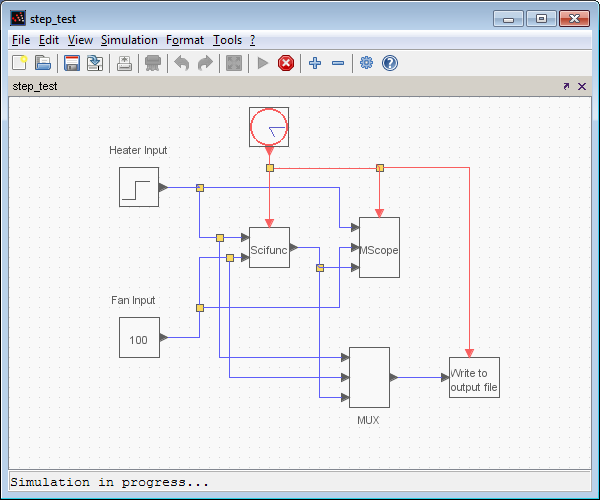
\includegraphics[width=\linewidth]{Step-test_manual/step.png}
\caption{Xcos for this experiment}
\label{xcos_st}
\end{figure}

\begin{figure}
\centering
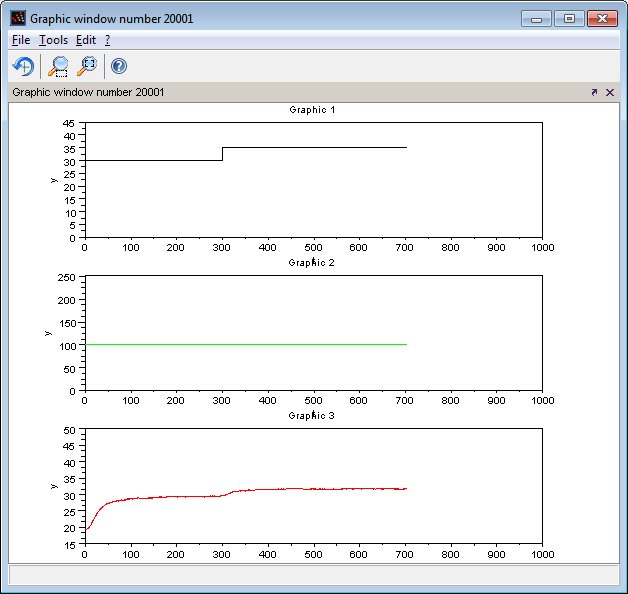
\includegraphics[width=\linewidth]{Step-test_manual/step_graph.png}
\caption{Graph shows Heater current , Fan speed and Output Temperature}
\label{fig:scope_st}
\end{figure}
We have used Scilab and Xcos as an interface for sending and receiving data. Xcos diagram is shown in Figure \ref{xcos_st}. Heater current and fan speed are the two inputs for this system. They are given in percentage of maximum. These inputs can be varied by the setting the properties of input block's properties in Xcos. The plots of their amplitude versus no. of collected samples are also available on the scope windows. The output temperature profile, as read by the sensor, is also plotted. The data acquired in the process is stored on the local drive and is available to the user for further calculations.

\section{Step by step procedure to perform Step Test}
The procedure to perform a step test is exactly the same as explained in Chapter \ref{sercomm}. In the {\tt step\_test.xcos} file, a block named {\tt write to output file} is used to make a log of the data generated during the experiment. Open the block's parameters to change the name of the file generated. Apply a step change of say 5 percent to the heater at operating point of 30 percent of heater after 300 seconds. This means that the block parameters of the step input block will have {\tt Step time = 300}, {\tt Initial value = 30} and {\tt Final value = 35}. Keep the fan input constant at 50 percent. Start the experiment and let it continue until you see the temperature almost reaching the steady state. 
\begin{table}
\begin{verbatim}
 0.100E+00  0.300E+02  0.100E+03  0.195E+02
 0.200E+00  0.300E+02  0.100E+03  0.195E+02
.
.
 0.704E+03  0.350E+02  0.100E+03  0.318E+02
 0.704E+03  0.350E+02  0.100E+03  0.318E+02
\end{verbatim}
\caption{Step data obtained after performing the Step Test}
\label{stepdata}
\end{table}
Referring to data file thus obtained as shown in Tabel \ref{stepdata}, the first column in this table denotes time. The second column in this table denotes heater current. It start at 30 and increases with a step size of 5 units. The third column denotes the fan speed. It has been held constant at 50 percent. The fourth column refers to the value of temperature.


\section{Determination of First order transfer function}
Identification of the transfer function of a system is quite important since it helps us to represent the physical system, mathematically. Once the transfer function is obtained one can acquire the response of the system for various inputs without actually applying them to the system.

Consider the standard first order transfer function given below
\begin{align}
G(s) &= \frac{ C(s)}{ R(s)}\label{1}\\
G(s)&=\frac 1{\tau s+1}\label{std_fo}                           
\intertext{Rewriting the Equation, we get}
C(s)  &= \frac {R(s)}{\tau s + 1}\label{rw_std_fo}
\intertext{A step is given as an input to the first order system. The Laplace Transform of a step function is$ \frac 1{s}$. Hence, substituting $ R(s) = \frac 1{s}$ in equation \ref{rw_std_fo}, we obtain}
C(s) & = \frac 1{\tau s + 1}\frac 1{s}\label{sub_rs}\\
\intertext{Solving $C(s)$ using partial fraction expansion, we get}
C(s) &= \frac1{s} - \frac {1}{s + \frac1 \tau}\label{pf}
\intertext{Taking the Inverse Laplace transform of equation \ref{pf}, we get}
c(t)&= 1 - e^{\frac {-t}\tau }\label{lti} 
\end{align}
from the above equation it is clear that for t=0 the value of c(t) is zero. For t= $\infty$, c(t) approaches unity. Also as the value of \textquoteleft t\textquoteright becomes equal to $\tau$, the value of c(t) becomes 0.632. The $\tau$ is called as the time constant and represents the speed of response of the system. But it should be noted that, the smaller the time constant, the faster the system response.\\
By getting the value of $\tau$, one can identify the transfer function of the system. 

Consider the system to be first order. We try to fit a first order transfer function of the form
\begin{align}       
G(s) &= \frac K{\tau s + 1}\label{7}
\intertext{to single board heater system.  Because the transfer function approach uses deviation variables,$ G(s)$ denotes the Laplace transform, of the gain of the system between the change in heater current and the change in the system temperature. Let the change in the heater current be denoted by $\Delta u$.  We denote both the time domain and the Laplace transform variable by the same lower case variable. Let the change in temperature be denoted by $y$.Suppose that the current changes by a step of size $u$.Then, we obtain the following relation between the current and the temperature.} 
y(s) &= G(s)u(s)\\ 
y(s)&= \frac K{\tau s + 1}{\frac  {\Delta u}{{s}}}
\intertext {Note that $\Delta$ u is the height of the step and hence is a constant. On inversion, we obtain}
y(s)&= K[1 - e^{\frac{-t}\tau}]\Delta u
\end{align}
Copy the step test data file to the folder {\tt Kp-tau-order1}. Change the scilab working directory to {\tt Kp-tau-order1} folder under {\tt Step\_Analysis} folder. Open the file {\ttfamily firstorder.sce} and put the name of the data file (with extention) in the filename field. Save and run this code and obtain the plot as shown in figure \ref{firstorder_output}. This code uses the routines {\ttfamily label.sci} and {\ttfamily costf\_1.sci}
\begin{figure}
\centering
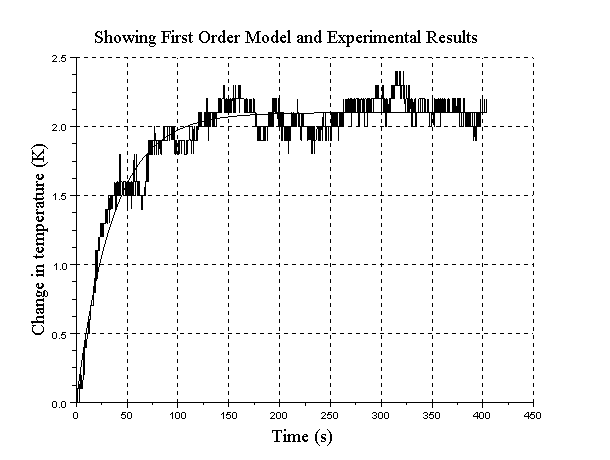
\includegraphics[width=\linewidth]{Step-test_manual/forder_fit.png}
\caption{Output of the scilab code \ttfamily firstorder.sce}
\label{firstorder_output}
\end{figure}

\begin{align}
\intertext{The plot thus obtained is reasonably good. See the Scilab console to get the values of $\tau$ and $K$. The figure \ref {console} shows a screen shot of the same. We obtain $\tau$ = 35.61087, K = 0.4201. The transfer function obtained here is at the operating point of 30 pwm of heat. If the experiment is repeated at a different operating point, the transfer function obtained will be different. The gain will correspondingly be more at a higher operating point. This means that the plant is faster at higher temperature. Thus the transfer function of the plant varies with the operating point.
Let the transfer function we obtain in this experiment be denoted as $G_s$.We obtain}
G_s(s) =  \frac{0.4201}{35.61s+1} \label{12}
\end{align}
\begin{figure}
\centering
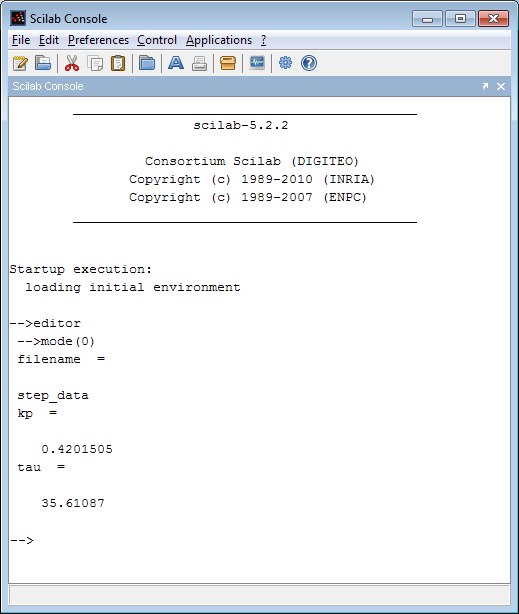
\includegraphics[width=\linewidth]{Step-test_manual/forder_console.png}
\caption{The value of time constant and gain as shown on the console by firstorder.sce}
\label{console}
\end{figure}


\section{Determination of second order transfer function}
In this section, we explore the efficacy of a second order model of the form
\begin{align}
G(s) & = \frac K{(\tau_1s+1)(\tau_2s+1)} \label{eq:step-1100} 
\intertext{The response of the system to a step input of height
  $\Delta u$ is given by}
y(s) & = \frac K{(\tau_1s+1)(\tau_2s+1)} \frac{\Delta u}s 
\label{eq:step-1200} 
\end{align}

Splitting this into partial fraction expansion, we obtain
\begin{align*}
y(s) & = \frac K{\tau_1\tau_2} \frac 1
{\left(s+\dfrac 1{\tau_1}\right)\left(s+\dfrac 1{\tau_2}\right)} =
\frac A s + \frac B{s+\dfrac 1{\tau_1}} + \frac C{s+\dfrac 1{\tau_2}}
\intertext{Through heaviside expansion method, we determine the
  coefficients:}
A & = K \\
B & = -\frac{K\tau_1}{\tau_1-\tau_2} \\
C & = \frac{K\tau_2}{\tau_1-\tau_2}
\end{align*}

On substitution and inversion, we obtain
\begin{align}
y(t) & = K\left[ 1 - \frac 1{\tau_1-\tau_2}
\left( \tau_1 e^{-t/\tau_1} - \tau_2 e^{-t/\tau_2} \right)
\right] \label{eq:step-1300}
\end{align}

We have to determine three parameters, $K$, $\tau_1$ and $\tau_2$
through optimization.  Once again, we follow a procedure identical to the first order model.  The only difference is that we now have to determine three parameters. Scilab code \\{\tt secondorder.sce} does these calculations and outputs a the gain and two time constants. Again change the scilab working diectory to the folder {\tt Kp-tau-order2}. Copy the step test data file in this folder. Run the code {\tt secondorder.sce} with the appropriate data file name. The plot shown in \ref{sorder} is obtained.  It corresponds to the following transfer function with the parameters written at the top of the plot.
\begin{align}
G_{s}(s) & = \frac {0.420}{(34.4s+1)(1s+1)}
\label{eq:step-1400}
\end{align}

\begin{figure}
\centering
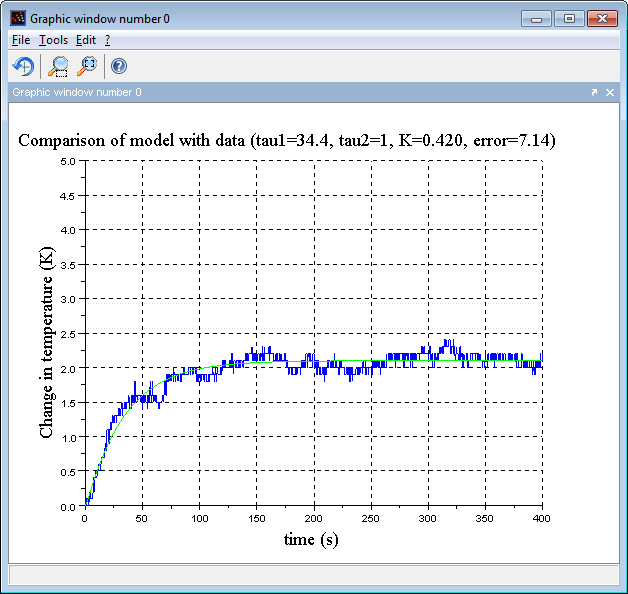
\includegraphics[width=\linewidth]{Step-test_manual/Sorder_fit.png}
\caption{Output of the scilab code \ttfamily secondorder.sce}
\label{sorder}
\end{figure}

The fit is much better now.  In particular, the initial inflexion is well captured by this second
order transfer function.


\section{Discussion}
We summarize our findings now. For the firstorder analysis the gain is 0.4201 and the time constant $\tau$ is 35.61 sec. For the second order analysis, the initial inflexion is well captured with the two time constants $\tau_1$=34.4, $\tau_2$= 1 and gain = 0.420. Negative steps can also be introduced to make the experiment more informative. One can even need not keep a particular input constant. By varying both the inputs, one can imagine it to be like a step varying disturbance signal.
 
\section{Conducting Step Test on SBHS, virtually}
The step by step procedure for conducting an experiment virtually is explained in section \ref{vlabsexpt}. The required .sce file is {\tt stepc.sce}.  You will find this file in the {\tt StepTest} directory under {\tt virtual} folder. Please note that the analysis code of step test data obtained by a virtual experiment is slightly different. The procedure to use the analysis code however remains the same as explained earlier. To do a first order analysis, one has to use the file {\tt firstorder\_virtual.sce}. Similarly, {\tt secondorder\_virtual.sce} for second order analysis. You will find this file in the {\tt StepTest} directory under {\tt virtual} folder. The necessary codes are listed in the section \ref{stepcodes}.


\section{Scilab Code}\label{stepcodes}
\begin{code}
\ccaption{label.sci}{\ttfamily label.sci}
\lstinputlisting{Scilab/local/Step_Analysis/Kp-tau-order1/label.sci}
\end{code}

\begin{code}
\ccaption{costf\_1.sci}{\ttfamily costf\_1.sci}
\lstinputlisting{Scilab/local/Step_Analysis/Kp-tau-order1/costf_1.sci}
\end{code}


\begin{code}
\ccaption{firstorder.sce}{\ttfamily firstorder.sce}
\lstinputlisting{Scilab/local/Step_Analysis/Kp-tau-order1/firstorder.sce}
\end{code}

\begin{code}
\ccaption{costf\_2.sci}{\ttfamily costf\_2.sci}
\lstinputlisting{Scilab/local/Step_Analysis/Kp-tau-order2/costf_2.sci}
\end{code}

\begin{code}
\ccaption{order\_2\_heater.sci}{\ttfamily order\_2\_heater.sci}
\lstinputlisting{Scilab/local/Step_Analysis/Kp-tau-order2/order_2_heater.sci}
\end{code}

\begin{code}
\ccaption{secondorder.sce}{\ttfamily secondorder.sce}
\lstinputlisting{Scilab/local/Step_Analysis/Kp-tau-order2/secondorder.sce}
\end{code}

\begin{code}
\ccaption{ser\_init.sce}{\ttfamily ser\_init.sce}
\lstinputlisting{Scilab/local/Step_test/ser_init.sce}
\end{code}

\begin{code}
\ccaption{step\_test.sci}{\ttfamily step\_test.sci}
\lstinputlisting{Scilab/local/Step_test/step_test.sci}
\end{code}

\begin{code}
\ccaption{stepc.sce}{\ttfamily stepc.sce}
\lstinputlisting{Scilab/virtual/StepTest/stepc.sce}
\end{code}

\begin{code}
\ccaption{steptest.sci}{\ttfamily steptest.sci}
\lstinputlisting{Scilab/virtual/StepTest/steptest.sci}
\end{code}

\begin{code}
\ccaption{firstorder\_virtual.sce}{\ttfamily firstorder\_virtual.sce}
\lstinputlisting{Scilab/virtual/Step_Analysis/Kp-tau-order1/firstorder_virtual.sce}
\end{code}

\begin{code}
\ccaption{secondorder\_virtual.sce}{\ttfamily secondorder\_virtual.sce}
\lstinputlisting{Scilab/virtual/Step_Analysis/Kp-tau-order2/secondorder_virtual.sce}
\end{code}











